%% Evaluation paper prepared for ACM Digital Threats: Research and Practice (DTRAP), acmart template.
%% Every number comes from a results file; captions give the path in the released repository.
%% Before submission: confirm the DTRAP author guidelines (template variant, abstract length, review mode).
\documentclass[acmlarge,screen,review]{acmart}

\usepackage{etoolbox}
\AtBeginEnvironment{table}{\linespread{1}\selectfont}
\usepackage{booktabs}
\usepackage{tabularx}
\newcolumntype{Y}{>{\raggedright\arraybackslash}X}
\usepackage{multirow}
\usepackage{pifont}
\newcommand{\cmark}{\ding{51}}

\newcommand{\todo}[1]{\textcolor{blue}{[TODO: #1]}}

\acmJournal{DTRAP}
\setcopyright{none}
\settopmatter{printacmref=false}
\renewcommand\footnotetextcopyrightpermission[1]{}

\begin{document}
\sloppy

\title[When Does Attack Knowledge Help Learned Intrusion Detectors?]{When Does Attack Knowledge Help Learned Intrusion
Detectors? A Pre-registered Evaluation of Detection, Explanation and Blast-Radius Prediction on Public Attack Datasets}

\author{Margarita Baimel Lerman}
\email{baimelrita@gmail.com}
\affiliation{%
  \institution{Tallinn University of Technology (TalTech)}
  \city{Tallinn}
  \country{Estonia}}
\author{Eduard Petlenkov}
\affiliation{%
  \institution{Tallinn University of Technology (TalTech)}
  \city{Tallinn}
  \country{Estonia}}
\author{Dmitry Baimel}
\affiliation{%
  \institution{SCE -- Shamoon College of Engineering}
  \city{Beer-Sheva}
  \country{Israel}}
\renewcommand{\shortauthors}{Baimel Lerman et al.}

\begin{abstract}
Security operations combine learned detectors with explicit attack knowledge such as MITRE ATT\&CK. We ask when this
knowledge improves a learned detector, whether alerts can be explained in ATT\&CK terms, and whether the next
compromised host can be predicted. All methods, splits, metrics and pass/fail gates were pre-registered before the
test data were opened, across nine public datasets of emulated or red-team attacks. On network flows, a pooled
autoencoder set a strong baseline (host-day AUC 0.960 vs.\ 0.673 for per-host detectors on OpTC). On host provenance,
fusing an ATT\&CK rule prior with a learned detector reached 7 of 10 process-centric Windows attacks within ten
alerts, where the learned detector alone found none; a confirmatory check on CARBANAKv2 reached the attack within
three alerts in every seed. On Linux, FreeBSD and Android the learned detector led. A negative control shows that the
gains come from rules marking the attack's processes, a measurable criterion for when to fuse. Grouping
reconstruction error by ATT\&CK channel identified the attack stage well above chance on Unraveled. On LANL, host
popularity proved a strong predictor of the next compromised host. Code, plans and results are released as research
infrastructure.
\end{abstract}

\begin{CCSXML}
<ccs2012>
 <concept><concept_id>10002978.10002997.10002999</concept_id>
  <concept_desc>Security and privacy~Intrusion detection systems</concept_desc>
  <concept_significance>500</concept_significance></concept>
 <concept><concept_id>10010147.10010257</concept_id>
  <concept_desc>Computing methodologies~Machine learning</concept_desc>
  <concept_significance>300</concept_significance></concept>
 <concept><concept_id>10002944.10011123.10011130</concept_id>
  <concept_desc>General and reference~Evaluation</concept_desc>
  <concept_significance>300</concept_significance></concept>
</ccs2012>
\end{CCSXML}
\ccsdesc[500]{Security and privacy~Intrusion detection systems}
\ccsdesc[300]{Computing methodologies~Machine learning}
\ccsdesc[300]{General and reference~Evaluation}

\keywords{intrusion detection, provenance, MITRE ATT\&CK, explainability, lateral movement, pre-registration,
evaluation}

\maketitle



\section{Introduction}\label{sec:intro}
Security operations centres combine two kinds of evidence: learned detectors, which flag behaviour that differs from
the past, and explicit attack knowledge, typically detection rules mapped to MITRE ATT\&CK
\cite{mitre2019ttphunting,mitre2026cti}. Research on learned detectors has moved quickly, from graph neural networks
over provenance graphs \cite{cheng2024kairos,jia2024magic,jiang2025orthrus,ren2025aptmgl} to temporal link prediction
for lateral movement \cite{king2022euler,xu2024argus,khoury2024jbeil}. Recent re-evaluations temper the reported
progress: in one framework, a simple neural network matches the state of the art on most DARPA datasets
\cite{bilot2025simpler,pidsmaker2026}, and lateral-movement detectors that reported near-perfect scores perform poorly
under a fair protocol \cite{larroche2026fair}. Knowledge-based systems
\cite{milajerdi2019holmes,hassan2019nodoze,hassan2020rapsheet,milajerdi2019poirot} predate these learned detectors.
Whether explicit attack knowledge still adds to a modern learned detector, and under which conditions, has not been
measured.

The question matters in practice. A rule prior costs engineering effort and analyst attention; if it adds noise on
some telemetry, fusing it everywhere lowers the number of attacks an analyst reaches within a fixed alert budget. It
also matters for method: machine learning for security has a record of results that do not survive careful
evaluation \cite{sommer2010outside,arp2022dos,pendlebury2019tesseract}, so a claim that knowledge helps should be
tested against criteria fixed in advance.

This paper reports a sequence of pre-registered experiments that began as the development of one model for
detection, ATT\&CK-level explanation and blast-radius prediction. Because plans, gates and test splits were fixed
before the test data were opened, every outcome, including those in which simpler baselines prevailed over our models,
is an unbiased measurement. Together they answer four questions:
\begin{description}
\item[RQ1] Do structured, per-host label-free detectors beat simple pooled detectors on public network data?
\item[RQ2] When does an explicit ATT\&CK prior improve a learned provenance detector under an analyst budget?
\item[RQ3] Which explanation method identifies the attack stage of an alert?
\item[RQ4] Can the next compromised host be predicted from authentication data beyond host popularity?
\end{description}
The four questions probe one thesis: the value of explicit attack knowledge is conditional; it depends on the
telemetry, on how the attack is represented in it, and on the task. RQ1 establishes what label-free detection
achieves on network telemetry without explicit knowledge; RQ2 to RQ4 test knowledge for detection, explanation and
prediction. Table~\ref{tab:summary} summarises the answers.

\begin{table}[!htbp]
\centering\footnotesize
\caption{Summary of findings. Numbers are from the pre-registered runs; seed ranges and intervals are given in the
corresponding sections.}
\label{tab:summary}
\setlength{\tabcolsep}{3pt}
\begin{tabularx}{\textwidth}{@{}p{0.7cm}>{\raggedright\arraybackslash}p{2.2cm}YY@{}}
\toprule
RQ & Answer & Key evidence & Value for practice and research \\
\midrule
RQ1 & Pooled baseline best & OpTC host-day AUC 0.960 for a pooled autoencoder vs.\ 0.673 for per-host channels,
consistent over six seeds & a strong, cheap default; per-host models need longer history \\
RQ2 & Yes, when rules cover the attack & Fusion reached 7 of 10 ATLASv2 attacks, the OpTC h051 attack and, as a
confirmatory check, the CARBANAKv2 attack (within 3 alerts in every seed) within 10 alerts (learned detector alone:
none); on DARPA TC E3 the learned detector led (4 of 6 attacks within 50 alerts) &
a measurable criterion for fusion: rule coverage of attack processes; random-target rules give no gain \\
RQ3 & Partly & Reconstruction-error grouping 0.563 vs.\ chance 0.263 on Unraveled in every seed; held-out OpTC shows
which explainers need validation & a simple, model-native explainer and a ground truth for validating others \\
RQ4 & Popularity is the bar & recall@100: PageRank 0.150, credential exposure 0.140, degree 0.131; all 13--19 times
random & a cheap prioritisation and the benchmark for propagation models \\
\bottomrule
\end{tabularx}
\end{table}

Beyond these answers, the study is designed as infrastructure and foundational evidence for further research on
machine-learning-based threat detection: it fixes a protocol, reference baselines and open tooling against which new
detectors, knowledge sources and explanation methods can be tested. The contributions are:
\begin{enumerate}
\item a pre-registered evaluation across nine public attack datasets (OpTC counted once, with a network view and a host
view; the three DARPA TC E3 sub-datasets counted separately), with all deviations and every outcome reported
(Appendix~\ref{app:prereg});
\item evidence on when a rule prior helps a learned provenance detector: where the rules cover the processes of
the attack, as shown by a negative control with content-free rules, a per-attack analysis and a confirmatory check on
a dataset whose ground truth was opened only after the rules were fixed, and not where attacks
appear as network connections or where the rules do not match the platform (Section~\ref{sec:rq2});
\item a ground-truth comparison of ATT\&CK-level explainers with per-dataset intervals and seed variability
(Section~\ref{sec:rq3});
\item evidence, with intervals, that host popularity is a strong benchmark for predicting the next compromised host
on LANL (Section~\ref{sec:rq4});
\item research infrastructure for ML-based threat detection: a reusable evaluation protocol (pre-registered
gates, budget- and attack-level metrics, within-host and negative controls, seed repetitions); open code that derives
ground truth, rule points and features from the nine public datasets; all plans, development logs and result files;
and Velox-lite, a disk-light, CPU-only re-implementation of the Velox detector validated against the original. New
detectors, knowledge sources and explainers can thus be compared with ours on commodity hardware;
\item foundational evidence on which later work can build: the reference baselines that a new method must
beat (a pooled autoencoder for network detection, host popularity for the next compromised host) and the conditions
under which explicit attack knowledge adds to a learned detector.
\end{enumerate}
Section~\ref{sec:related} reviews related work and Section~\ref{sec:design} the study design. Sections~\ref{sec:rq1}
to~\ref{sec:rq4} answer the four questions, Section~\ref{sec:discussion} discusses implications for practice and
threats to validity, and Section~\ref{sec:conclusion} concludes.

\section{Background and related work}\label{sec:related}
\subsection{Learned provenance-based detection}
Provenance-based intrusion detection systems (PIDS) learn the normal behaviour of system entities from audit logs;
Li et al.\ survey their architecture and evaluation \cite{li2021provsurvey}. UNICORN compares graph sketches of
whole-system provenance with models of benign behaviour \cite{han2020unicorn}; ATLAS learns attack sequences for
investigation \cite{alsaheel2021atlas}. Kairos scores events with a temporal graph encoder-decoder and summarises
attacks as compact graphs \cite{cheng2024kairos}. MAGIC and APT-MGL use masked graph representation learning
\cite{jia2024magic,ren2025aptmgl}, and Flash combines word2vec semantics of node attributes with a graph neural
network \cite{rehman2024flash}. Orthrus targets the quality of attribution, the effort an analyst spends per alert
\cite{jiang2025orthrus}. Bilot et al.\ re-implemented eight such systems in one framework, found that a simple neural
network (Velox) reaches state-of-the-art detection on five of seven DARPA datasets, and showed that published ground
truth over-counted malicious nodes \cite{bilot2025simpler}; PIDSMaker distributes the framework, pre-processed datasets
and consistent labels \cite{pidsmaker2026}. Suarez-Roman and Tapiador show that node-level metrics can misrepresent
how well a PIDS recovers the structure of an attack \cite{suarezroman2025structure}; we therefore report attack-level
outcomes (attacks reached within a budget, alerts needed to reach each attack) next to node counts.

\subsection{Knowledge-based detection and threat intelligence}
HOLMES maps low-level events to ATT\&CK-like tactics and correlates them into high-level scenario graphs
\cite{milajerdi2019holmes}. NoDoze propagates anomaly scores along provenance dependencies to triage the alerts of
existing detectors \cite{hassan2019nodoze}. RapSheet builds tactical provenance graphs from endpoint detection alerts
\cite{hassan2020rapsheet}. POIROT searches audit logs for a graph that aligns with a query graph of attack behaviour
taken from threat-intelligence reports \cite{milajerdi2019poirot}, and automated mapping of unstructured threat
intelligence to ATT\&CK techniques supplies such knowledge at scale \cite{li2024ttpmapping}. These systems combine
knowledge with anomaly evidence, but they were evaluated before the current generation of learned PIDS and under
different protocols; none measures the marginal value of knowledge on top of a modern learned detector.

\subsection{Network-level and lateral-movement detection}
Anomaly detection for networks faces a closed-world problem: benign traffic is diverse and attacks are rare
\cite{sommer2010outside}, and labelled network datasets suffer from shortcuts and leakage \cite{arp2022dos}.
Lateral-movement detectors model authentication or flow graphs
\cite{king2022euler,bowman2020lateral,xu2024argus,khoury2024jbeil,king2026cybergfm}, and Larroche shows that their
reported performance on LANL and OpTC does not hold under a fair protocol \cite{larroche2026fair}.

\subsection{Explanation methods in security}
Feature attribution with SHAP is the most common way to explain anomaly detectors \cite{antwarg2021shap}; concept-based
models expose human-meaningful intermediate variables \cite{koh2020cbm,yuksekgonul2023posthoc}. Warnecke et al.\
proposed general and security-specific criteria for explanation methods and found that the methods differ widely on
security tasks \cite{warnecke2020explain}. Evaluations of ATT\&CK-level explanations against ground-truth attack
stages remain rare; RQ3 provides one.

\subsection{Evaluation methodology}
Spatial and temporal bias inflate results in malware classification \cite{pendlebury2019tesseract}, a catalogue of
pitfalls covers machine learning in security more broadly \cite{arp2022dos}, and in time-series anomaly detection
simple baselines rival deep models once evaluation is made rigorous \cite{sarfraz2024quovadis}. Pre-registration,
standard in parts of the empirical sciences, separates confirmatory from exploratory analysis by fixing hypotheses and
analyses before the data are seen \cite{nosek2018prereg}; we apply it to intrusion detection, with pass/fail gates.

\subsection{Positioning}
Table~\ref{tab:related} places this study among the closest work. Learned detectors and their re-evaluations do not
test explicit attack knowledge \cite{bilot2025simpler}; knowledge-based systems predate the learned detectors
considered here and were evaluated on other data and protocols
\cite{milajerdi2019holmes,hassan2019nodoze,hassan2020rapsheet,milajerdi2019poirot}; Larroche evaluates
lateral-movement detectors only \cite{larroche2026fair}. We ask the complementary question: when does a rule prior add
to a modern learned detector under one fixed budget-based protocol, across telemetry types and operating systems, and
how do explanations and propagation predictions compare in the same protocol?

\begin{table}[!htbp]
\centering\footnotesize
\caption{Closest related work. \cmark: addressed; ($\cmark$): partly; --: not addressed. Columns: learned
detector; explicit attack knowledge (rules, ATT\&CK or threat intelligence); explanation or attribution evaluated
against ground truth (Expl.); lateral movement or next-host prediction; one protocol across several telemetry types
or operating systems (Cross-tel.); pass/fail criteria fixed before testing (Pre-reg.). Based on each paper's own description.}
\label{tab:related}
\setlength{\tabcolsep}{4pt}
\begin{tabular}{p{4.2cm}cccccc}
\toprule
Work & Learned & Knowl. & Expl. & Lateral & Cross-tel. & Pre-reg. \\
\midrule
HOLMES \cite{milajerdi2019holmes} & -- & \cmark & -- & -- & -- & -- \\
POIROT \cite{milajerdi2019poirot} & -- & \cmark & -- & -- & -- & -- \\
NoDoze \cite{hassan2019nodoze} & ($\cmark$) & ($\cmark$) & -- & -- & -- & -- \\
RapSheet \cite{hassan2020rapsheet} & -- & \cmark & -- & -- & -- & -- \\
UNICORN, Kairos, MAGIC, Flash \cite{han2020unicorn,cheng2024kairos,jia2024magic,rehman2024flash} & \cmark & -- & -- & -- & -- & -- \\
Orthrus \cite{jiang2025orthrus} & \cmark & -- & ($\cmark$) & -- & -- & -- \\
Bilot et al.\ \cite{bilot2025simpler} & \cmark & -- & -- & -- & \cmark & -- \\
Euler, Bowman et al., Argus, Jbeil \cite{king2022euler,bowman2020lateral,xu2024argus,khoury2024jbeil} & \cmark & -- & -- & \cmark & -- & -- \\
Larroche \cite{larroche2026fair} & \cmark & -- & -- & \cmark & ($\cmark$) & -- \\
This study & \cmark & \cmark & \cmark & \cmark & \cmark & \cmark \\
\bottomrule
\end{tabular}
\end{table}

\section{Study design}\label{sec:design}
Figure~\ref{fig:design} gives an overview: three telemetry types feed the four questions, and every phase follows the
same pre-registration protocol.
\begin{figure}[t]
\centering
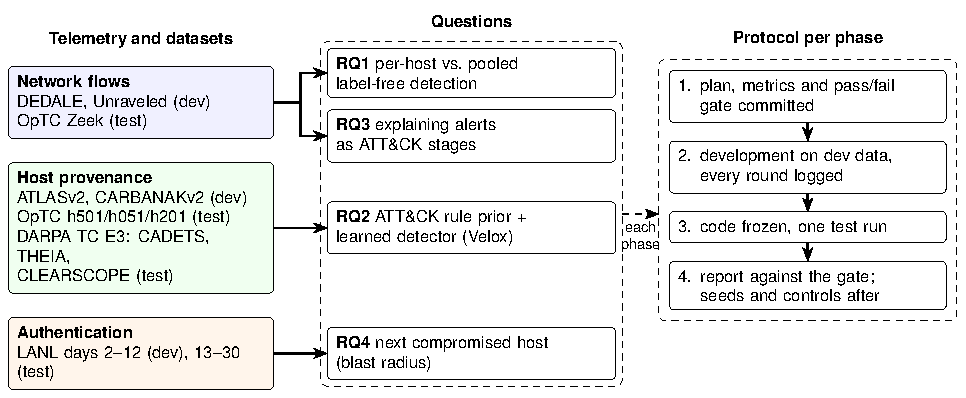
\includegraphics[width=\textwidth]{figures/fig_design.pdf}
\Description{Diagram with three columns: datasets grouped by telemetry type, the four research questions they feed, and the four-step pre-registration protocol applied to every phase.}
\caption{Study overview. Development (dev) and test data per telemetry type, the question each feeds, and the
protocol that every phase followed. Seed repetitions and controls were run after the pre-registered test runs, each
with its own plan committed beforehand.}
\label{fig:design}
\end{figure}
\subsection{Pre-registration protocol}
Each phase followed the same protocol.
\begin{enumerate}
\item A plan fixing methods, data splits, metrics and a pass/fail gate was committed to version control before the
phase's test data were downloaded or opened.
\item Development used only data designated as development data, and every development round, including rounds
that were rejected, was logged.
\item Code was frozen and committed before the single test run.
\item Any deviation forced by the environment was recorded before the affected run.
\end{enumerate}
Results are reported against the gate as committed, including gates that passed for the wrong reason. Data used
for testing in one phase became development data in later phases. Appendix~\ref{app:prereg} lists the commits.

\subsection{Datasets}
None of the datasets is a recorded operational intrusion. Attack activity is emulated or performed by red teams in
testbeds, with generated or simulated benign activity; Unraveled is explicitly semi-synthetic \cite{myneni2023unraveled},
and LANL combines benign activity from a real corporate network with red-team events \cite{kent2015lanl}. We therefore
call our evidence public benchmark evidence. By ``nine datasets'' we mean DEDALE, Unraveled, OpTC, ATLASv2,
CARBANAKv2, the three DARPA TC E3 sub-datasets (CLEARSCOPE, CADETS, THEIA) and LANL; OpTC is used with a network view
(Zeek) and a host view (three hosts).
\begin{table}[!htbp]
\centering\footnotesize
\caption{Datasets and their roles: DEDALE \cite{dedale2026}, Unraveled \cite{myneni2023unraveled}, DARPA OpTC
\cite{darpa2020optc}, ATLASv2 \cite{riddle2024atlasv2}, CARBANAKv2 and DARPA TC E3 as pre-processed by PIDSMaker
\cite{pidsmaker2026}, LANL \cite{kent2015lanl}. Ground truth as distributed (PIDSMaker for provenance data).}
\label{tab:data}
\setlength{\tabcolsep}{3pt}\footnotesize
\begin{tabularx}{\textwidth}{@{}YYYYY@{}}
\toprule
Dataset & Telemetry & Attack origin & Role & Attacks / GT nodes \\
\midrule
DEDALE & Zeek flows & emulated APT, virtualised testbed & RQ1 development & 1 campaign \\
Unraveled & NFStream flows & semi-synthetic, emulated groups & RQ1 test (P2), development (P3) & 2 groups \\
DARPA OpTC (Zeek) & Zeek flows & DARPA red team, emulated enterprise & RQ1 test (P3) & 3 days \\
ATLASv2-EDR & Windows provenance & lab engagements & RQ2 development & 10 / 48 \\
CARBANAKv2-EDR & Windows+Linux provenance & lab emulation & RQ2 confirmatory check & 1 / 229 \\
OpTC h501, h051, h201 & Windows provenance & DARPA red team & RQ2 test (Phase 2) & 1 / 749; 1 / 114; 1 / 2{,}905 \\
DARPA TC E3: CLEARSCOPE, CADETS, THEIA & Android, FreeBSD, Linux provenance & DARPA red team, testbed & RQ2 test (Phase 3) & 1 / 41; 3 / 72; 2 / 118 \\
LANL & authentication & red team in a real corporate network & RQ4 (dev days 2--12, test 13--30) & 194 / 107 first compromises \\
\bottomrule
\end{tabularx}
\end{table}

\subsection{Methods}
\subsubsection{Network level (RQ1, RQ3)}
Per host and hour we computed features grouped into ATT\&CK-inspired channels: reconnaissance, command and control
(including rare destinations and beacon regularity), lateral movement, exfiltration and volume.
Our detector scores each feature against the host's own history with a one-sided empirical tail (ECOD-style) and
calibrates channel scores with cross-fitted conformal p-values; a GraphSAGE link-prediction model scores internal
connections for the lateral-movement channel. Baselines are pooled ECOD, Isolation Forest and an autoencoder on the
same features, plus flow volume.

\subsubsection{Host level (RQ2)}
\begin{itemize}
\item Learned detector: Velox, the simple state-of-the-art PIDS \cite{bilot2025simpler}. It predicts each
event's type from word2vec embeddings of the two endpoints; a node's score is its maximum event loss. It was run via
PIDSMaker where the disk allowed; otherwise we used Velox-lite, our re-implementation that computes features on the
fly. On ATLASv2, Velox-lite reaches AUC 0.836 against 0.864 for PIDSMaker's Velox.
\item Knowledge prior: points per process from deterministic rules written from public ATT\&CK and Sigma
knowledge. They cover command-line patterns, and document or network-facing parents spawning interpreters or
living-off-the-land binaries. There are separate rule sets for Windows and for Linux/FreeBSD.
\item Fusion: a weighted sum of the learned detector's percentile and the points ($\lambda=0.1$), or
interleaving of the two rankings.
\end{itemize}

\subsubsection{Blast radius (RQ4)}
We rank the hosts that will be compromised next using degree, breadth-first neighbours, personalized PageRank and
credential exposure. Credential exposure counts the users with a session on a host after its compromise and the
hosts they log on to.

\subsection{Use of AI-assisted tools in the research process}
The research idea, the architecture, the design of the experiments and the structure of the paper are the
authors' own: the first author conceived them, defined the research questions, chose the datasets and directed the
study throughout. Claude Code (Anthropic) was used under the authors' direction as an implementation tool: to write
and run the experiment code and to compute the tables and figures from the result files. The authors approved each plan and gate before the corresponding test data
were opened and reviewed all results. All plans, code and result files are released; each table cites its source
file, so every number can be traced and re-computed independently.

\subsection{Metrics}
Because a security analyst inspects a bounded number of alerts, the primary metrics are budget-based: the number of
attacks with at least one ground-truth node among the top $k$ alerts, and the number of ground-truth nodes found
there, for $k$ = 10, 25, 50, 100, 250 and 500. Supporting metrics are the AUC and AP of the node ranking, the number of
alerts needed to reach each attack (rank of its first ground-truth node), host-day and host-hour AUC and detection
under a daily alert budget at the network level, attribution accuracy for RQ3 (share of attack host-hours whose
explained channel matches the ground-truth stage), and recall@$k$ of first-compromise targets for RQ4.

\subsection{Controls and statistical analysis}
Every comparison is made under one alert budget per dataset, and the gates are evaluated on the original seed only.
Beyond the gates we used:
\begin{itemize}
\item within-host controls, comparing a host's attack periods with its own normal periods, so that a detector
cannot pass by ranking host roles (RQ1);
\item seed repetitions for every learned component, five additional seeds each (Appendix~\ref{app:seeds});
\item a negative control for the rule prior: the same rule points re-assigned to random processes of the test
population, 1{,}000 draws per dataset and seed (RQ2);
\item cluster bootstrap intervals, resampling host-days for RQ3 and test days for RQ4 (1{,}000 and 10{,}000
draws);
\item exact permutation tests for cross-dataset correlations, Wilcoxon signed-rank tests for paired per-attack
comparisons, and Holm correction over the tests of the mechanism analysis (RQ2).
\end{itemize}
Analyses added after a phase's test run were planned in writing before they were computed and are labelled
exploratory.

\section{RQ1: label-free detection on network flows}\label{sec:rq1}
% dep/pilot/RESULTS_P1.md, RESULTS_P2.md, RESULTS_P3_OPTC.md
\begin{table}[!htbp]
\centering\small
\caption{OpTC (Zeek, held-out test), host-day AUC. Results file: \texttt{network\_level/results/RESULTS\_P3\_OPTC.md}.}
\label{tab:rq1}
\begin{tabular}{lc}
\toprule
Method & Host-day AUC \\
\midrule
Tactic channels + pooled ECOD (ours, P3) & 0.673 \\
Pooled autoencoder & \textbf{0.960} \\
Pooled ECOD & 0.896 \\
Pooled Isolation Forest & 0.876 \\
Flow volume & 0.296 \\
\bottomrule
\end{tabular}
\end{table}
Three pre-registered pilots tested increasingly structured label-free detectors.
\begin{itemize}
\item P1, DEDALE. The gate passed (recall at 10 alerts per day 0.727 vs.\ 0.438 at random). A within-host check
showed that the model mainly ranked host roles, which is why within-host controls became part of the protocol.
\item P2, Unraveled. Per-host baselines found 25\% of attacked host-days at 5 alerts per day, 3.8 times random and
above volume and host-prior baselines, below the 50\% target; flow volume had a higher host-hour AUC (0.805 vs.\
0.761).
\item P3, OpTC. Adding a GNN lateral-movement channel, beacon and rare-destination features and fusion with pooled
ECOD gave the best model on Unraveled (development); on the held-out OpTC test the pooled autoencoder was stronger
(Table~\ref{tab:rq1}).
\end{itemize}
On the two OpTC days with a meaningful ground truth, the pooled autoencoder reached host-day AUC 0.897 and 0.953
against 0.584 and 0.716 for our model. The OpTC Zeek sensor saw 60 internal connections in a sample hour, all ICMP,
so no network-level method could observe lateral movement there, a sensor property that OpTC studies should account for. We repeated the whole P3 pipeline with five more
seeds: each seed re-trains the GNN channel (whose output is also a feature of the pooled baselines), the autoencoder
and the Isolation Forest. Our model scored 0.673 in all six seeds; the GNN channel alone scored 0.513 in every seed, so
it does not drive the OpTC ranking. The autoencoder ranged from 0.960 to 0.991 (median 0.985) and was the best method in
every seed; the Isolation Forest ranged from 0.857 to 0.892, and ECOD is deterministic (0.896). On Unraveled
(development) the tactic channels without the ECOD fusion had the highest host-day AUC in five of six seeds
(0.881--0.891).

\subsection{Answer to RQ1}
Pooled models set the bar. A pooled autoencoder was the strongest label-free detector on held-out data in every
seed, which makes a simple, cheap model a strong default; per-host structure needs more than the four days of history
per host available here to add value.

\section{RQ2: attack knowledge and learned provenance detection}\label{sec:rq2}
% dep/reach/RESULTS_PHASE2.md, RESULTS_PHASE3.md, DEVLOG.md
\begin{table}[!htbp]
\centering\small
\caption{Attacks detected within 10 / 25 / 50 alerts. Learned detector: Velox-lite. Interleave on OpTC is a
post-hoc development result (it was pre-registered only for E3). Results files:
\texttt{provenance/results/RESULTS\_PHASE2.md}, \texttt{RESULTS\_PHASE3.md}.}
\label{tab:rq2}
\begin{tabular}{llcccc}
\toprule
Dataset & Role & Learned & Knowledge & Sum & Interleave \\
\midrule
ATLASv2 (10 attacks) & dev & 0/0/0 & 2/8/9 & 7/8/9 & 1/4/8 \\
OpTC h501 & test & 1/1/1 & 0/1/1 & 0/1/1 & (1/1/1) \\
OpTC h051 & test & 0/0/0 & 1/1/1 & 1/1/1 & (1/1/1) \\
OpTC h201 & test & 0/1/1 & 0/0/1 & 0/0/1 & (0/0/1) \\
CLEARSCOPE E3 & test & 0/0/0 & 0/0/0 & 0/0/0 & 0/0/0 \\
CADETS E3 (3) & test & 0/0/2 & 0/0/0 & 0/0/0 & 0/0/0 \\
THEIA E3 (2) & test & 1/1/1 & 0/0/0 & 0/0/0 & 1/1/1 \\
\bottomrule
\end{tabular}
\end{table}
\begin{figure}[t]
\centering
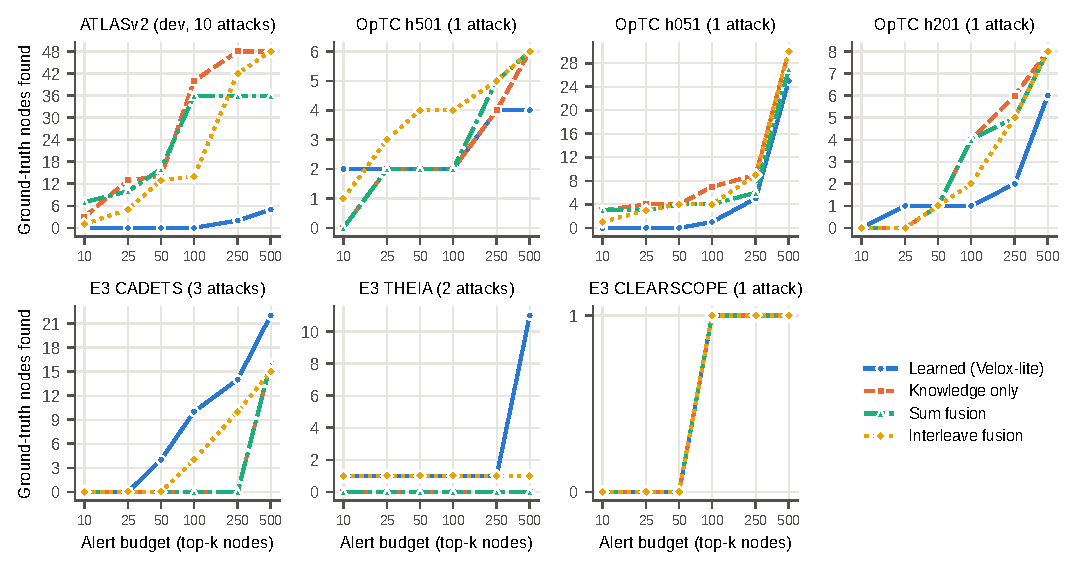
\includegraphics[width=\textwidth]{figures/fig_budget.pdf}
\Description{Eight line charts, one per dataset, showing ground-truth nodes found against the alert budget for the learned detector, knowledge only, sum fusion and interleave fusion.}
\caption{Ground-truth nodes found within the top-$k$ alerts. The learned detector is Velox-lite in every panel.
ATLASv2 is development data; interleave on ATLASv2 and OpTC is a post-hoc development result (it was pre-registered
only for DARPA TC E3). Exact values in Table~\ref{tab:rq2} and the results files.}
\label{fig:budget}
\end{figure}

\subsection{Development}
On ATLASv2 the learned detector alone found no attack within 50 alerts. The fused ranking found 7 of 10 within
10 alerts (5--7 over five Velox-lite seeds, median 7; the learned detector alone found none within 50 alerts in any
seed). Because the Windows rules were partly written with ATLASv2 in view, CARBANAKv2, whose ground truth was not
inspected before the rules were fixed, serves as the confirmatory check (Section~\ref{sec:carbanak}).

\subsection{Phase 2 (OpTC, Windows)}
Results differed by host, which shows what the prior can see.
\begin{itemize}
\item h051: the attack is process-centric (59 of 114 ground-truth nodes are processes). Knowledge found it within
10 alerts; the learned detector needed 100.
\item h501 and h201: the ground truth is dominated by network-connection nodes (700 of 749 and 2{,}858 of 2{,}905),
which a process-level prior cannot score; there the learned detector reached the attacks first.
\end{itemize}
The gate, which required fusion to match the learned detector on every host, was not met on h201 at 25 alerts;
pooled over the three hosts, fusion found more than twice as many ground-truth nodes within 50 alerts (7 vs.\ 3,
seed 0).

\subsection{Phase 3 (DARPA TC E3, Linux/FreeBSD/Android)}
Development on all previously seen data selected interleaving as the primary fusion, because it never lost an
attack that either ranking found early. On the three E3 datasets the learned detector led: 3 of 6 attacks within 50
alerts against 1 for interleaving and 0 for knowledge alone (seed 0), which marks where rule sets need
platform-specific work.
\begin{itemize}
\item THEIA: the Linux rules marked 13{,}291 test processes.
\item CLEARSCOPE (Android): no process matched any rule.
\item CADETS: the learned detector reached AUC 0.979 (seed 0; median over five seeds 0.969).
\end{itemize}

\subsection{Seed variability}
Velox-lite was repeated with four more seeds on all six test datasets (plan committed before the runs). The gate
outcome was identical in all five seeds, so the conclusions are robust to the detector's seed-to-seed variation
(Appendix~\ref{app:seeds}, Table~\ref{tab:seeds}). Figure~\ref{fig:budget} shows the pattern for ground-truth nodes
across all budgets.

\subsection{Mechanism}
To find out why the prior helped on some datasets and not on others, we fixed four hypotheses in a plan before
computing the quantities below, and a negative control in a second plan; no model was re-trained (frozen node scores of all five seeds, one fusion definition
for every dataset). Table~\ref{tab:mech} gives the per-dataset quantities.
\begin{table}[!htbp]
\centering\footnotesize
\caption{Mechanism analysis over the seven provenance datasets with a learned detector, medians over five seeds.
Process share: share of ground-truth (GT) nodes that are processes. Coverage: share of GT processes marked by the
rules. Selectivity: share of all test processes marked (needs no labels). Gain: fused minus learned GT nodes within
50 alerts. AUC: learned detector's node AUC. Alerts L / F: alerts needed to reach an attack, learned / fused (median over
attacks). Results files: \texttt{mechanism/RESULTS\_MECHANISM.md}, \texttt{round4/RESULTS\_NEGATIVE\_CONTROL.md}.}
\label{tab:mech}
\setlength{\tabcolsep}{3pt}
\begin{tabular}{lcccccc}
\toprule
Dataset & Proc.\ share & Coverage & Select. & AUC & Gain & Alerts L / F \\
\midrule
ATLASv2 (dev) & 1.00 & 1.00 & 0.017 & 0.843 & +26 & 2{,}894 / 7 \\
OpTC h051 & 0.52 & 0.12 & 0.006 & 0.859 & +4 & 105 / 4 \\
OpTC h501 & 0.03 & 0.09 & 0.008 & 0.723 & 0 & 5 / 12 \\
OpTC h201 & 0.01 & 0.12 & 0.009 & 0.728 & 0 & 13 / 41 \\
CADETS & 0.54 & 0.00 & 0.003 & 0.969 & $-5$ & 35 / 271 \\
THEIA & 0.81 & 0.00 & 0.125 & 0.630 & $-1$ & 166 / 1{,}418 \\
CLEARSCOPE & 0.02 & 0.00 & 0.000 & 0.162 & 0 & 196 / 196 \\
\midrule
CARBANAKv2 (confirmatory) & 1.00 & 0.50 & 0.030 & 0.342 & +5 & 3{,}035 / 2 \\
\bottomrule
\end{tabular}
\end{table}
\begin{itemize}
\item Content-free rules (negative control). We re-assigned the observed rule points to randomly chosen
processes of the same test population (same number of marked processes and same point values; 1{,}000 draws per
dataset and seed). On ATLASv2 and h051 the real rules beat every control in every seed (observed gain $+26$ and $+4$
nodes; control median 0; one-sided $p\le0.002$ in all ten dataset-seeds). On h501 the real rules lost nothing where
random rules lost two nodes ($p=0.01$--$0.02$ per seed). On CADETS the real rules lost exactly as much as random
rules ($-5$ vs.\ $-5$), and on THEIA slightly more: the E3 losses are the cost of adding unrelated points to a ranking,
not of any particular rule. The gain on Windows therefore comes from what the rules mark, not from the fusion
arithmetic.
\item Coverage, not process share, went with the gain (H2). Over the seven datasets the Spearman correlation
between the rules' coverage of ground-truth processes and the gain was 0.81 (exact permutation $p=0.043$; 0.13 after
Holm correction over five tests). The share of processes in the ground truth was unrelated to the gain
($\rho=0.07$, $p=0.88$): CADETS and THEIA are process-centric, but the Linux rules covered none of their attack
processes.
\item The learned detector's strength did not predict the gain (H3): $\rho=0.07$, $p=0.88$; a detector with a good
AUC still benefits from rules that cover the attack.
\item Representation (H1). On h501 and h201, restricted to ground-truth processes, the prior found as many
within 50 alerts as the learned detector (2 vs.\ 2 and 1 vs.\ 1): it matched it on the process part of the
attack; the rest is recorded as network connections, which call for network-level evidence.
\item Per attack (H4). On the 11 process-centric Windows attacks (ATLASv2 and h051), fusion reached every attack
earlier than the learned detector (median 5 vs.\ 2{,}698 alerts; Wilcoxon $p=0.001$, 0.005 after Holm). On the other 8
attacks the learned detector was earlier on 7 and tied on 1 (median 34 vs.\ 271; $p=0.016$, 0.06 after Holm). Ten of
the 11 Windows attacks come from ATLASv2 (development data); the held-out h051 attack and the CARBANAKv2 check
(Section~\ref{sec:carbanak}) show the same effect.
\item Coverage needs labelled activity. Selectivity on unlabelled data did not separate the cases (CADETS 0.3\%,
h051 0.6\%), so coverage should be measured on replayed emulations of the expected techniques, a step operations
teams can run routinely.
\end{itemize}
The negative control and the per-attack comparison hold within each dataset and carry the main evidence; the
cross-dataset correlation adds support (exploratory; no gate depends on it).

\subsection{Confirmatory check on CARBANAKv2}\label{sec:carbanak}
Before running the learned detector on CARBANAKv2 we committed two predictions derived from the mechanism (rule
coverage 0.50): fusion finds more ground-truth nodes within 50 alerts than the learned detector (median over five
seeds), and reaches the attack first in at least four of five seeds. Both held. The learned detector ranked the attack
below benign activity (AUC 0.33--0.39) and found no ground-truth node within 50 alerts in any seed; fusion found 5
(2--12) and reached the attack within 1--3 alerts in every seed, against 321--6{,}387 for the learned detector. The
real rules beat rules with random targets in every seed ($p\le0.042$). Dropping any one rule family
(leave-one-out over six families) still reached the attack within a median of 2 alerts, so the gain does not rest on
a single pattern; the document-parent rule, the one refined after inspecting ATLASv2, marked no process here.

\subsection{Answer to RQ2}
Yes, when the rules cover the attack. An explicit ATT\&CK prior improves a learned provenance detector where its
rules mark the processes of the attack: there it beats rules of equal selectivity with random targets and reaches
attacks in a handful of alerts. Process-centric ground truth is necessary but not sufficient, and the strength of the
learned detector did not predict the benefit. Where the rules mark nothing of the attack, the learned detector should
lead, so fusion is best applied selectively. This turns the decision to fuse into a measurable test.

\section{RQ3: explaining alerts in ATT\&CK terms}\label{sec:rq3}
% dep/explain/RESULTS_E1.md, accuracy_ci.json
\begin{table}[!htbp]
\centering\footnotesize
\caption{Attribution accuracy (explained channel is a ground-truth channel), point estimate and 95\% bootstrap
interval over host-days (1,000 resamples). Number of attack host-hours (host-days): Unraveled 645 (60), OpTC days 1--2
102 (34), DEDALE 12 (10), pooled 759 (104). Results file: \texttt{explanation/results/accuracy\_ci.json}.}
\label{tab:rq3}
\setlength{\tabcolsep}{3pt}\footnotesize
\begin{tabular}{@{}p{3.1cm}cccc@{}}
\toprule
Explainer & Unraveled & OpTC (held out) & DEDALE & Pooled \\
\midrule
Autoencoder error grouped by ATT\&CK channel & 0.563 (0.43--0.68) & 0.294 (0.19--0.42) & 0.750 & 0.530 (0.42--0.64) \\
Occlusion (autoencoder) & 0.397 (0.30--0.51) & 0.314 (0.23--0.41) & 0.833 & 0.393 (0.31--0.48) \\
TreeSHAP (Isolation Forest) & 0.357 (0.23--0.49) & 0.412 (0.26--0.57) & 0.500 & 0.366 (0.25--0.48) \\
KernelSHAP (autoencoder) & 0.341 (0.21--0.46) & 0.069 (0.02--0.14) & 0.750 & 0.311 (0.20--0.42) \\
Calibrated tactic channels (ours, pre-registered) & 0.254 (0.15--0.39) & 0.373 (0.25--0.53) & 0.583 & 0.275 (0.19--0.38) \\
Chance (uniform over four channels) & 0.263 (0.26--0.27) & 0.341 (0.32--0.37) & 0.354 & 0.275 (0.27--0.28) \\
\bottomrule
\end{tabular}
\end{table}
Each attack host-hour was explained by the channel with the largest attribution, aggregated over that channel's
features. A host-hour can have several ground-truth channels, and an explanation counts as correct if it names any of
them, so the chance level differs per dataset (0.26--0.35; Appendix~\ref{app:impl} gives the mapping from the
datasets' stage labels to channels and the chance computation).

The pooled figure is dominated by one dataset: 645 of 759 host-hours (85\%) come from Unraveled. We therefore base
the answer on the per-dataset results.
\begin{itemize}
\item Unraveled: grouping the autoencoder's reconstruction error by channel (0.563) is clearly above chance
(0.263; the intervals do not overlap), and above occlusion, TreeSHAP and KernelSHAP. Over six seeds it stayed above
chance in every seed (0.41--0.65) and was the best explainer in four (Table~\ref{tab:rq3seeds}); its lead over the
other explainers therefore depends on the seed, its distance from chance does not.
\item OpTC (held out): this harder, held-out case separates the methods from chance only for KernelSHAP, which
is below it (0.069, interval 0.02--0.14, against chance 0.341), and below chance in five of six seeds (median 0.181). The
reconstruction-error grouping (0.294) does not replicate its Unraveled advantage there; over seeds it ranged from 0.28
to 0.68 and was above chance in three of six, so on OpTC its accuracy depends on the trained autoencoder, a
reason to validate explainers per environment.
\item DEDALE (12 host-hours) is too small to separate the methods.
\end{itemize}
Our pre-registered calibrated channels reached chance level on Unraveled and slightly above chance on OpTC and
DEDALE. The reconstruction-error grouping, added as a baseline, is the most promising method (exploratory). The
pre-registered faithfulness metric divides by near-zero occlusion drops and is not reported. The E1 gate was not met
in any seed.

\subsection{Answer to RQ3}
Partly. Grouping an autoencoder's reconstruction error by ATT\&CK channel identified the attack stage well above
chance on Unraveled in every seed, which makes it a simple, model-native candidate for ATT\&CK-level explanation. Its
weaker held-out result on OpTC, and KernelSHAP's below-chance accuracy there, show that explanations must be validated
in each environment before analysts rely on them; the released ground-truth stages make that validation possible.

\section{RQ4: predicting the next compromised host}\label{sec:rq4}
% dep/reach/RESULTS_L3_LANL.md
\begin{table}[!htbp]
\centering\small
\caption{LANL, test days 13--30 (107 first compromises). Results file: \texttt{blast\_radius/RESULTS\_L3\_LANL.md}.}
\label{tab:rq4}
\begin{tabular}{lccc}
\toprule
Method & recall@10 & recall@50 & recall@100 \\
\midrule
Random & 0.001 & 0.004 & 0.008 \\
Degree & 0.056 & 0.103 & 0.131 \\
Personalized PageRank & 0.047 & 0.112 & 0.150 \\
Credential exposure (pre-registered) & 0.056 & 0.103 & 0.140 \\
\bottomrule
\end{tabular}
\end{table}

On LANL, red-team activity spans days 2--30. One computer is the source of 701 of 749 compromise events, and a
single day (day 9) holds 170 of the 194 development targets. On that day the attacker used 43 accounts, 40 of which
had sessions on already compromised hosts beforehand. So did 9{,}008 other users, which diluted the
credential-exposure signal. On the test days, credential exposure tied with degree at 50 hosts (0.103) and was
marginally above it at 100 (0.140 vs.\ 0.131), short of the pre-registered margin. Personalized PageRank, which was below degree in
development, was best on the test days (0.150 at 100). Resampling the six test days that contain new targets
(10{,}000 draws), the difference from degree at 100 hosts was $+0.019$
($-0.031$ to $+0.044$) for Personalized PageRank and $+0.009$ (0.000 to $+0.031$) for credential exposure. 

\subsection{Answer to RQ4}
Host popularity is the bar. All methods are 13--19 times better than random, and none exceeds host popularity
beyond its interval. Popularity is therefore a strong, cheap prioritisation for incident responders and the
benchmark that propagation models must beat.

\section{Discussion}\label{sec:discussion}
\subsection{The thesis, restated}
Across the four questions, explicit attack knowledge was never uniformly good or bad. In detection (RQ2) its value
depended on whether the rules marked the processes of the attack: where they did (process-centric Windows attacks),
fusion beat rules of equal selectivity with random targets and reached attacks in a handful of alerts; where they
marked nothing of the attack (DARPA TC E3), the learned detector led; and where the attack was recorded mainly as
network connections (OpTC h501, h201), network-level evidence is needed. As explanation (RQ3), the most promising
signal came from the learned model itself. For prediction (RQ4), host popularity was as informative as credential
knowledge.

\subsection{Implications for security operations}
\begin{itemize}
\item Test a rule prior's coverage before fusing it. Replay emulations of the techniques the organisation
expects and measure the share of attack processes the rules mark. Neither the rules' selectivity on unlabelled data
nor the learned detector's AUC predicted the benefit in our data.
\item Treat rule sets as platform-specific. The Linux rules marked none of the E3 attack processes; a rule set
that works on Windows process trees says nothing about other platforms until its coverage is measured there.
\item Fuse selectively and keep both rankings. Where coverage is zero, fusion displaces the learned detector's
top alerts; keeping the learned ranking visible next to a fused list avoids that cost.
\item Pair process rules with network-level models for attacks that appear mainly as connections.
\item Validate explanations in each environment. Reconstruction-error grouping is a promising default, and each
explainer, KernelSHAP included, should be checked against labelled incidents before analysts act on it.
\item Use simple baselines as the bar. A pooled autoencoder for network detection and host popularity for the
next compromised host were the methods to beat; a more complex method should be adopted only if it beats them on the
organisation's own data.
\end{itemize}

\subsection{Implications for research}
A gate passed in P1 because the model ranked host roles; within-host controls, comparing a host's attack days with its
own normal days, caught the error. Development results were consistently more favourable than test results (Unraveled
vs.\ OpTC in P3, ATLASv2 vs.\ E3 in Phases 2--3), and pre-registration made these gaps visible instead of tunable. A
pooled result can hide dataset dominance: the explanation advantage came from one dataset that supplied 85\% of the
host-hours. Negative controls distinguish what a component contributes from what the evaluation arithmetic produces:
on E3, real and random rules lost the same amount. We therefore recommend budget- and attack-level metrics,
per-dataset results with intervals, several seeds, and negative controls as standard reporting for detection studies.

\subsection{Threats to validity}
\begin{itemize}
\item Compute and seeds. All experiments ran on a CPU-only machine; Velox used embedding size 32 and Velox-lite
replaced it on OpTC and E3 (AUC 0.836 vs.\ 0.864 for the original on ATLASv2). Every learned component was repeated
with five more seeds (Appendix~\ref{app:seeds}); no gate outcome changed, while explainer rankings did, so explainers
should be compared over several seeds. The GNN training was bit-reproducible on OpTC but not between runs on DEDALE
and Unraveled, which the seed study covers.
\item Number of attacks. The datasets contain 1--10 attacks each, so results are reported per attack and per
dataset with intervals; the cross-dataset correlation of the mechanism analysis is exploratory.
\item External validity. Attacks are emulated or red-team activity in testbeds (LANL adds real benign activity), so
the conclusions concern public benchmarks; the protocol transfers directly to an organisation's own data.
\item Unit of analysis. Bootstrap intervals resample host-days, because host-hours of one host are correlated.
\item Rule design. The Windows rules were partly written with ATLASv2 in view; held-out evidence for the Windows
effect comes from OpTC h051 and from the confirmatory check on CARBANAKv2, whose ground truth was opened only
after the rules were fixed (Section~\ref{sec:carbanak}). The E3 attack reports were known in outline; no
dataset-specific names were used.
\item Containment and ethics. No malicious code was executed and no new attack activity was generated: all
attack data are public recordings of past red-team or emulated activity, used under the providers' terms (LANL after
its registration form). No personal data beyond the providers' anonymised identifiers were processed.
\item Transparency. Plans, gates, development logs, code and all result files are released; every table names its
results file.
\item Deviations. $\lambda$ was set by the pre-registered default rule after disk limits stopped the CARBANAKv2
Velox runs.
\end{itemize}

\section{Conclusion}\label{sec:conclusion}
Across nine public attack datasets, and with every gate fixed in advance, the most consistent findings were simple:
\begin{itemize}
\item a pooled autoencoder was the strongest label-free network detector on held-out data and is the baseline to beat;
\item grouping reconstruction error by ATT\&CK channel identified the attack stage above chance on Unraveled in every
seed, and held-out results show that explainers need per-environment validation;
\item explicit attack knowledge helped learned provenance detectors where its rules marked the attack's processes, a
condition that can be measured before deployment and that held on a confirmatory dataset;
\item host popularity predicted the next compromised host as well as more complex methods and is the benchmark for
propagation models.
\end{itemize}
These results argue for measuring a knowledge prior's coverage of attack processes on the target telemetry before
deploying it, and for evaluating detectors under analyst budgets, with within-host and negative controls and several
seeds. We release all plans, logs, code and results as infrastructure for further research on ML-based threat
detection: new detectors can be evaluated against the same baselines and gates, new knowledge sources (for example
rules derived automatically from threat intelligence) against the same negative control, and new explanation methods
against the same ground-truth stages.

\section*{Author contributions}
Margarita Baimel Lerman: conceptualization, methodology, investigation, formal analysis, data curation,
visualization, writing (original draft, review and editing), project administration. Eduard Petlenkov and Dmitry
Baimel: supervision, methodology, writing (review and editing).

\section*{Competing interests}
The authors declare that they have no known competing financial interests or personal relationships that could have
appeared to influence the work reported in this paper.

\section*{Use of generative AI}
The research idea, the architecture, the design of the experiments and the structure of the paper are the authors'
own. Under the authors' direction, Claude Code (Anthropic) was used as an implementation tool for software
development, running the experiments, data analysis and figure generation, and Claude (Anthropic) as a writing
assistant for drafting and editing text. All plans, gates, results and
text were reviewed by the authors, who take full responsibility for the content.

\section*{Data availability}
All datasets used are public: DEDALE (Recherche Data Gouv, \url{https://doi.org/10.57745/Y5JLDG}); Unraveled
(\url{https://gitlab.com/asu22/unraveled}); DARPA OpTC (\url{https://github.com/FiveDirections/OpTC-data});
ATLASv2-EDR, CARBANAKv2-EDR, the OpTC host datasets and DARPA TC E3 as pre-processed by PIDSMaker
(\url{https://github.com/ubc-provenance/PIDSMaker}); and the LANL Comprehensive, Multi-Source Cyber-Security Events
(\url{https://csr.lanl.gov/data/cyber1/}). Code, pre-registrations, development logs and all result files are available
at \url{https://github.com/baimelrita-rgb/attack-knowledge-ids-eval}.

\begin{acks}
This research did not receive any specific grant from funding agencies in the public, commercial, or not-for-profit
sectors.
\end{acks}

\bibliographystyle{ACM-Reference-Format}
\bibliography{refs}

\appendix
\section{Implementation details}\label{app:impl}
\subsection{Data splits}
\subsubsection{Network level}
Days are UTC; the unit is the host-hour of Zeek or NFStream flows.
\begin{table}[!htbp]\centering\footnotesize\setlength{\tabcolsep}{3pt}
\caption{Train / calibration / test days for the network-level experiments. Train and calibration days contain no attack flow.}
\begin{tabularx}{\textwidth}{@{}lYYY@{}}
\toprule
Dataset & Train & Calibration & Test \\
\midrule
DEDALE (green zone) & 2024-12-24 -- 2025-01-02 & 2025-01-03 -- 2025-01-05 & 2025-01-06 -- 2025-01-19 \\
Unraveled & 2021-05-28 -- 2021-06-04 & 2021-06-05 -- 2021-06-07 & 2021-06-08 -- 2021-07-06 \\
OpTC (Zeek) & 2019-09-16 -- 2019-09-19 & 2019-09-20 -- 2019-09-22 & 2019-09-23 -- 2019-09-25 \\
\bottomrule
\end{tabularx}
\end{table}
\subsubsection{Provenance level}
The splits are PIDSMaker's defaults for each dataset.
\begin{table}[!htbp]\centering\footnotesize\setlength{\tabcolsep}{3pt}
\caption{Train / validation / test dates for the host-level experiments: first and last day, and the number of days actually used in parentheses (the days of a split need not be contiguous).}
\begin{tabularx}{\textwidth}{@{}lYYY@{}}
\toprule
Dataset & Train & Validation & Test \\
\midrule
ATLASv2-EDR & 2022-07-16 -- 18 (2\,d) & 2022-07-17 & 2022-07-19 -- 20 (2\,d) \\
CARBANAKv2-EDR & 2024-04-20 -- 29 (8\,d) & 2024-04-22 -- 26 (2\,d) & 2024-04-30 -- 2024-05-10 (7\,d) \\
OpTC h501 & 2019-09-19 -- 21 (3\,d) & 2019-09-22 & 2019-09-23 -- 25 (3\,d) \\
OpTC h051 & 2019-09-19 -- 21 (3\,d) & 2019-09-22 & 2019-09-23 -- 25 (3\,d) \\
OpTC h201 & 2019-09-19 -- 21 (3\,d) & 2019-09-22 & 2019-09-23 -- 25 (3\,d) \\
CLEARSCOPE E3 & 2018-04-03 -- 10 (7\,d) & 2018-04-02 & 2018-04-11 -- 12 (2\,d) \\
CADETS E3 & 2018-04-02 -- 09 (7\,d) & 2018-04-10 & 2018-04-06 -- 13 (4\,d) \\
THEIA E3 & 2018-04-02 -- 08 (7\,d) & 2018-04-09 & 2018-04-10 -- 13 (3\,d) \\
\bottomrule
\end{tabularx}
\end{table}
LANL: development = days 2--12, test = days 13--30 of the red-team events (day index from the start of the data).

\subsection{Models and hyperparameters}
\begin{itemize}
\item Network features (per host-hour): flows out, distinct destination IPs and ports, share of failed
connections, new and rare external destinations (rare = contacted by at most two internal hosts before), beacon
regularity over 72\,h, bytes out and in, new admin-port edges, GNN edge surprise. Counts and bytes are transformed
with $\log(1+x)$; ratios are left unchanged. ``New'' means not seen on any earlier day.
\item Per-host tail model: one-sided empirical upper-tail probability of each feature against the host's own
training hours (all hosts' hours if the host has fewer than 24); channel score = most extreme feature (+0.01 $\times$
channel mean); conformal $p$-values from cross-fitted calibration (training days split by parity, plus the calibration
days); hour score $=-\log_{10}(\min_c p_c \times 6)$.
\item Pooled baselines: ECOD (pyod defaults); Isolation Forest (200 trees); autoencoder = scikit-learn
\texttt{MLPRegressor} with hidden layers (32, 8, 32), 300 iterations, on standardised features. Seed 42 unless stated.
\item GNN lateral channel: learnable 32-d node embeddings, two GraphSAGE-mean layers, MLP decoder over
(source, destination, port embedding of size 8); 300 epochs of Adam (learning rate 0.01, weight decay $10^{-4}$);
three random destinations and two random ports per observed triple as negatives; training days scored out of sample
by two models trained on alternate days; seed 42.
\item Velox / Velox-lite: PIDSMaker's Velox (tuned configuration, embedding size 32) and our re-implementation
(word2vec embeddings of node labels with PIDSMaker's tokenizer, size 32, 10 epochs; a linear layer to 128 dimensions;
source and destination projections to 256; dropout 0.5; one hidden layer; cross-entropy over the event type; 3 epochs
of Adam with learning rate $10^{-3}$ on at most 4 million sampled training events). Node score = maximum event loss.
\item Explanation baselines: KernelSHAP with 20 $k$-means background points and 200 samples; TreeSHAP on the
Isolation Forest; occlusion replaces a channel's features by their training medians; reconstruction-error grouping
takes the channel with the largest mean squared per-feature error.
\item Blast radius: logon weights $\log(1+n)\,e^{-\Delta d/7}$ over earlier days; PageRank restart 0.15, 50
iterations, undirected graph.
\end{itemize}

\subsection{Windows rule prior (process path or command line)}
Each matching rule adds one point to a process; process-creation events add two points to both endpoints when a
document, mail or browser process spawns an interpreter or living-off-the-land binary, and one point when an
interpreter spawns such a tool.
\begin{itemize}\footnotesize
\item \texttt{powershell.\allowbreak{}*\allowbreak{}(\allowbreak{}-\allowbreak{}enc|\allowbreak{}-\allowbreak{}e |\allowbreak{}encodedcommand|\allowbreak{}iex|\allowbreak{}invoke-\allowbreak{}expression|\allowbreak{}downloadstring|\allowbreak{}-\allowbreak{}nop|\allowbreak{}bypass)\allowbreak{}} $\rightarrow$ T1059.\allowbreak{}001
\item \texttt{\textbackslash\{\}\textbackslash\{\}powershell(\allowbreak{}\_ise)\allowbreak{}?\allowbreak{}\textbackslash\{\}.\allowbreak{}exe} $\rightarrow$ T1059.\allowbreak{}001
\item \texttt{\textbackslash\{\}\textbackslash\{\}cmd\textbackslash\{\}.\allowbreak{}exe} $\rightarrow$ T1059.\allowbreak{}003
\item \texttt{\textbackslash\{\}\textbackslash\{\}mshta\textbackslash\{\}.\allowbreak{}exe} $\rightarrow$ T1218.\allowbreak{}005
\item \texttt{\textbackslash\{\}\textbackslash\{\}rundll32\textbackslash\{\}.\allowbreak{}exe} $\rightarrow$ T1218.\allowbreak{}011
\item \texttt{\textbackslash\{\}\textbackslash\{\}regsvr32\textbackslash\{\}.\allowbreak{}exe} $\rightarrow$ T1218.\allowbreak{}010
\item \texttt{\textbackslash\{\}\textbackslash\{\}(\allowbreak{}wmic|\allowbreak{}wmiprvse)\allowbreak{}\textbackslash\{\}.\allowbreak{}exe} $\rightarrow$ T1047
\item \texttt{\textbackslash\{\}\textbackslash\{\}schtasks\textbackslash\{\}.\allowbreak{}exe} $\rightarrow$ T1053.\allowbreak{}005
\item \texttt{reg(\allowbreak{}\textbackslash\{\}.\allowbreak{}exe)\allowbreak{}?\allowbreak{} add .\allowbreak{}*\allowbreak{}\textbackslash\{\}\textbackslash\{\}run} $\rightarrow$ T1547.\allowbreak{}001
\item \texttt{certutil.\allowbreak{}*\allowbreak{}(\allowbreak{}urlcache|\allowbreak{}decode)\allowbreak{}} $\rightarrow$ T1105
\item \texttt{\textbackslash\{\}\textbackslash\{\}(\allowbreak{}whoami)\allowbreak{}\textbackslash\{\}.\allowbreak{}exe} $\rightarrow$ T1033
\item \texttt{\textbackslash\{\}\textbackslash\{\}(\allowbreak{}net1?\allowbreak{}|\allowbreak{}netstat)\allowbreak{}\textbackslash\{\}.\allowbreak{}exe} $\rightarrow$ T1087
\item \texttt{\textbackslash\{\}\textbackslash\{\}(\allowbreak{}ipconfig|\allowbreak{}arp|\allowbreak{}route)\allowbreak{}\textbackslash\{\}.\allowbreak{}exe} $\rightarrow$ T1016
\item \texttt{\textbackslash\{\}\textbackslash\{\}systeminfo\textbackslash\{\}.\allowbreak{}exe} $\rightarrow$ T1082
\item \texttt{\textbackslash\{\}\textbackslash\{\}tasklist\textbackslash\{\}.\allowbreak{}exe} $\rightarrow$ T1057
\item \texttt{vssadmin.\allowbreak{}*\allowbreak{}delete} $\rightarrow$ T1490
\item \texttt{\textbackslash\{\}\textbackslash\{\}psexe(\allowbreak{}c|\allowbreak{}svc)\allowbreak{}} $\rightarrow$ T1569.\allowbreak{}002
\item \texttt{\textbackslash\{\}\textbackslash\{\}mstsc\textbackslash\{\}.\allowbreak{}exe} $\rightarrow$ T1021.\allowbreak{}001
\item \texttt{lsass} $\rightarrow$ T1003.\allowbreak{}001
\item \texttt{\textbackslash\{\}\textbackslash\{\}(\allowbreak{}winword|\allowbreak{}excel|\allowbreak{}powerpnt|\allowbreak{}outlook)\allowbreak{}\textbackslash\{\}.\allowbreak{}exe} $\rightarrow$ T1566.\allowbreak{}001
\item \texttt{\textbackslash\{\}\textbackslash\{\}(\allowbreak{}wscript|\allowbreak{}cscript)\allowbreak{}\textbackslash\{\}.\allowbreak{}exe} $\rightarrow$ T1059.\allowbreak{}005
\item \texttt{\textbackslash\{\}\textbackslash\{\}bitsadmin\textbackslash\{\}.\allowbreak{}exe} $\rightarrow$ T1197
\end{itemize}

\subsection{Linux / FreeBSD / Android rule prior}
Same point scheme; parents are network-facing programs (browsers, mail clients, web, ssh and ftp servers), children
are shells, interpreters and download or discovery tools.
\begin{itemize}\footnotesize
\item \texttt{(\allowbreak{}\^{}|\allowbreak{}/\allowbreak{})\allowbreak{}(\allowbreak{}tmp|\allowbreak{}dev/\allowbreak{}shm|\allowbreak{}var/\allowbreak{}tmp)\allowbreak{}/\allowbreak{}[\^{} ]*\allowbreak{}} $\rightarrow$ T1059 exec from temp dir
\item \texttt{chmod\textbackslash\{\}s+\allowbreak{}(\allowbreak{}\textbackslash\{\}+\allowbreak{}x|\allowbreak{}[0-\allowbreak{}7]*\allowbreak{}7[0-\allowbreak{}7]*\allowbreak{})\allowbreak{}} $\rightarrow$ T1222.\allowbreak{}002
\item \texttt{base64\textbackslash\{\}s+\allowbreak{}(\allowbreak{}-\allowbreak{}d|\allowbreak{}-\allowbreak{}-\allowbreak{}decode)\allowbreak{}} $\rightarrow$ T1140
\item \texttt{(\allowbreak{}wget|\allowbreak{}curl)\allowbreak{}\textbackslash\{\}s+\allowbreak{}[\^{}|\allowbreak{}]*\allowbreak{}http} $\rightarrow$ T1105
\item \texttt{(\allowbreak{}curl|\allowbreak{}wget)\allowbreak{}[\^{}|\allowbreak{}]*\allowbreak{}\textbackslash\{\}|\allowbreak{}\textbackslash\{\}s*\allowbreak{}(\allowbreak{}ba)\allowbreak{}?\allowbreak{}sh} $\rightarrow$ T1059.\allowbreak{}004
\item \texttt{\textbackslash\{\}b(\allowbreak{}nc|\allowbreak{}ncat|\allowbreak{}netcat|\allowbreak{}socat)\allowbreak{}\textbackslash\{\}b.\allowbreak{}*\allowbreak{}(\allowbreak{}-\allowbreak{}e|\allowbreak{}-\allowbreak{}c|\allowbreak{}exec)\allowbreak{}} $\rightarrow$ T1059.\allowbreak{}004 reverse shell
\item \texttt{/\allowbreak{}etc/\allowbreak{}(\allowbreak{}passwd|\allowbreak{}shadow|\allowbreak{}sudoers)\allowbreak{}} $\rightarrow$ T1003.\allowbreak{}008
\item \texttt{crontab|\allowbreak{}/\allowbreak{}etc/\allowbreak{}cron} $\rightarrow$ T1053.\allowbreak{}003
\item \texttt{\textbackslash\{\}.\allowbreak{}ssh/\allowbreak{}authorized\_keys} $\rightarrow$ T1098.\allowbreak{}004
\item \texttt{\textbackslash\{\}b(\allowbreak{}whoami|\allowbreak{}id|\allowbreak{}uname -\allowbreak{}a|\allowbreak{}hostname|\allowbreak{}ifconfig|\allowbreak{}ip addr|\allowbreak{}netstat|\allowbreak{}ss -\allowbreak{})\allowbreak{}\textbackslash\{\}b} $\rightarrow$ T1033/\allowbreak{}T1082/\allowbreak{}T1016
\item \texttt{\textbackslash\{\}b(\allowbreak{}useradd|\allowbreak{}adduser|\allowbreak{}usermod)\allowbreak{}\textbackslash\{\}b} $\rightarrow$ T1136.\allowbreak{}001
\item \texttt{\textbackslash\{\}b(\allowbreak{}scp|\allowbreak{}sftp)\allowbreak{}\textbackslash\{\}b} $\rightarrow$ T1105
\item \texttt{insmod|\allowbreak{}modprobe} $\rightarrow$ T1547.\allowbreak{}006
\item \texttt{history\textbackslash\{\}s+\allowbreak{}-\allowbreak{}c|\allowbreak{}rm\textbackslash\{\}s+\allowbreak{}-\allowbreak{}rf\textbackslash\{\}s+\allowbreak{}/\allowbreak{}var/\allowbreak{}log|\allowbreak{}unset\textbackslash\{\}s+\allowbreak{}HISTFILE} $\rightarrow$ T1070
\end{itemize}

\subsection{Ground-truth channels for the explanation study}
An explanation counts as correct if the explained channel is among the ground-truth channels of the host-hour;
host-hours without a mappable channel are excluded. The chance level is the expected accuracy of choosing one of the
four channels uniformly at random, that is, the average of $|\mathrm{GT}\cap\{\text{recon, c2, lateral, exfil}\}|/4$
over the evaluated host-hours.
\begin{itemize}\footnotesize
\item DEDALE (ATT\&CK tactic ID): TA0043, TA0007 $\rightarrow$ recon; TA0011 $\rightarrow$ c2; TA0008 $\rightarrow$
lateral; TA0010 $\rightarrow$ exfil; TA0001, TA0009 $\rightarrow$ none.
\item Unraveled (stage): Reconnaissance $\rightarrow$ recon; Establish Foothold $\rightarrow$ c2; Lateral Movement
$\rightarrow$ lateral; Data Exfiltration $\rightarrow$ exfil; Cover up $\rightarrow$ none.
\item OpTC: flows to a documented attacker server $\rightarrow$ c2; report-timeline entries by keyword (scan
$\rightarrow$ recon; pivot, WMI, RDP, spread $\rightarrow$ lateral; exfiltrat, netcat $\rightarrow$ exfil).
\end{itemize}

\subsection{Values behind Figure~\ref{fig:budget}}
\begin{table}[!htbp]\centering\footnotesize\setlength{\tabcolsep}{3pt}
\caption{Ground-truth nodes found within the top-$k$ alerts (seed 0).}
\begin{tabular}{llcccccc}
\toprule
Dataset & Method & 10 & 25 & 50 & 100 & 250 & 500 \\
\midrule
ATLASv2 (dev) & Learned & 0 & 0 & 0 & 0 & 2 & 5 \\
 & Knowledge & 3 & 13 & 14 & 40 & 48 & 48 \\
 & Sum & 7 & 10 & 16 & 36 & 36 & 36 \\
 & Interleave & 1 & 5 & 13 & 14 & 42 & 48 \\
\midrule
OpTC h501 & Learned & 2 & 2 & 2 & 2 & 4 & 4 \\
 & Knowledge & 0 & 2 & 2 & 2 & 4 & 6 \\
 & Sum & 0 & 2 & 2 & 2 & 5 & 6 \\
 & Interleave & 1 & 3 & 4 & 4 & 5 & 6 \\
\midrule
OpTC h051 & Learned & 0 & 0 & 0 & 1 & 5 & 25 \\
 & Knowledge & 3 & 4 & 4 & 7 & 9 & 30 \\
 & Sum & 3 & 3 & 4 & 4 & 6 & 27 \\
 & Interleave & 1 & 3 & 4 & 4 & 9 & 30 \\
\midrule
OpTC h201 & Learned & 0 & 1 & 1 & 1 & 2 & 6 \\
 & Knowledge & 0 & 0 & 1 & 4 & 6 & 8 \\
 & Sum & 0 & 0 & 1 & 4 & 5 & 8 \\
 & Interleave & 0 & 0 & 1 & 2 & 5 & 8 \\
\midrule
CADETS E3 & Learned & 0 & 0 & 4 & 10 & 14 & 22 \\
 & Knowledge & 0 & 0 & 0 & 0 & 0 & 16 \\
 & Sum & 0 & 0 & 0 & 0 & 0 & 16 \\
 & Interleave & 0 & 0 & 0 & 4 & 10 & 15 \\
\midrule
THEIA E3 & Learned & 1 & 1 & 1 & 1 & 1 & 11 \\
 & Knowledge & 0 & 0 & 0 & 0 & 0 & 0 \\
 & Sum & 0 & 0 & 0 & 0 & 0 & 0 \\
 & Interleave & 1 & 1 & 1 & 1 & 1 & 1 \\
\midrule
CLEARSCOPE E3 & Learned & 0 & 0 & 0 & 1 & 1 & 1 \\
 & Knowledge & 0 & 0 & 0 & 1 & 1 & 1 \\
 & Sum & 0 & 0 & 0 & 1 & 1 & 1 \\
 & Interleave & 0 & 0 & 0 & 1 & 1 & 1 \\
\bottomrule
\end{tabular}
\end{table}

\section{Seed variability}\label{app:seeds}
The pre-registered decisions use one seed (seed~0 for Velox-lite, seed~42 for the network-level models). Two later
rounds, each with a plan committed before its runs (PLAN\_SEEDS.md, PLAN\_SEEDS2.md), repeated: Velox-lite with seeds
1--4 on the six test datasets and on ATLASv2; and the full RQ1 and RQ3 pipelines (GNN channel, pooled autoencoder and
Isolation Forest, explainers) with seeds 0--4 plus a re-run of seed 42. The re-run reproduced every OpTC number
exactly. On DEDALE and Unraveled the GNN training was not bit-reproducible between runs on our CPU, so the
development tables are one draw of that variation. On OpTC the learned detector's AUC on h201 ranged from 0.520 to
0.732 and the ground-truth nodes found on CADETS within 50 alerts from 2 to 15; on CLEARSCOPE its AUC was below 0.5 in
every seed (median 0.162).

\begin{table}[!htbp]
\centering\small
\caption{Pooled gate quantities over five seeds, median (min--max). Results file: \texttt{provenance/results/RESULTS\_SEEDS.md}.}
\label{tab:seeds}
\begin{tabular}{llccc}
\toprule
Phase & Quantity & Learned & Knowledge & Fusion \\
\midrule
E3 (3 datasets) & attacks within 50 alerts & 4 (3--5) & 0 (0--0) & 1 (1--3) \\
OpTC (3 hosts) & GT nodes within 50 alerts & 3 (2--3) & 7 (6--7) & 7 (6--7) \\
\bottomrule
\end{tabular}
\end{table}

\begin{table}[!htbp]
\centering\footnotesize
\caption{Attribution accuracy over six seeds (the original seed re-run and five more), median (min--max). Each seed
re-trains the GNN features, the autoencoder and the Isolation Forest and redraws the KernelSHAP samples. ``Best'' counts
the seeds in which the explainer had the highest accuracy. Results file: \texttt{network\_level/results/RESULTS\_SEEDS2.md}.}
\label{tab:rq3seeds}
\setlength{\tabcolsep}{3pt}
\begin{tabular}{@{}p{3.1cm}cccc@{}}
\toprule
Explainer & Unraveled & best & OpTC (held out) & best \\
\midrule
Autoencoder error grouped by channel & 0.513 (0.41--0.65) & 4/6 & 0.358 (0.28--0.68) & 3/6 \\
Occlusion (autoencoder) & 0.407 (0.34--0.53) & 1/6 & 0.324 (0.31--0.42) & 1/6 \\
TreeSHAP (Isolation Forest) & 0.364 (0.23--0.40) & 0/6 & 0.319 (0.19--0.42) & 1/6 \\
KernelSHAP (autoencoder) & 0.387 (0.23--0.61) & 1/6 & 0.181 (0.07--0.35) & 0/6 \\
Calibrated tactic channels (ours) & 0.251 (0.14--0.26) & 0/6 & 0.373 (0.37--0.37) & 1/6 \\
Chance & 0.263 & & 0.341 & \\
\bottomrule
\end{tabular}
\end{table}

\section{Pre-registrations, deviations and development logs}\label{app:prereg}
\begin{table}[!htbp]
\centering\footnotesize
\caption{Pre-registered phases. Plan = commit fixing methods and gate before the test data were opened; Result =
commit with the single test run.}
\label{tab:prereg}
\begin{tabularx}{\textwidth}{@{}YYllY@{}}
\toprule
Phase & Test data & Plan & Result & Gate \\
\midrule
P1 & DEDALE & 89564ee & adc3f59 & passed; post-hoc: wrong reason \\
P2 & Unraveled & d75eb3a & 2b7f7a6 & failed (item 1) \\
P3 & OpTC Zeek & dc15828, f525c58 & df382a9 & failed \\
E1 (explanation) & DEDALE, Unraveled, OpTC & 77573b9, a17fd2c & 8f75662 & failed \\
L3 (blast radius) & LANL days 13--30 & 5dc767f & 61e0217 & failed \\
Phase 2 & OpTC h501/h051/h201 & 5dc767f, 5a40f17 & df49584 & failed (h201 at 25) \\
Seeds 1--4 & six test datasets & 42bd3b9 & 7919f41 & same gate outcome in all seeds \\
Seeds, round 2 & OpTC, Unraveled, DEDALE, ATLASv2 & ad6a27a & 56ea3bd & same gate outcome in all seeds \\
Mechanism (RQ2) & seven provenance datasets & 533221d & 9f0c33e & exploratory; no gate \\
Controls and CARBANAKv2 check & provenance datasets, CARBANAKv2 & b79168d & 48989ed, c780587 & both predictions held \\
Phase 3 & DARPA TC E3 & 79841b9 & 8c07398 & failed \\
\bottomrule
\end{tabularx}
\end{table}
Deviations: Velox embedding size 32 and Velox-lite (disk limit; recorded in 5dc767f and 5a40f17 before the OpTC
runs); $\lambda=0.1$ by default rule after the CARBANAKv2 runs failed; LANL split changed before any blast-radius
run because red-team activity ends on day 30.


\end{document}
